\newpage

\section*{ $^{24}$Cu(n,p)$^{24}$Cu }

Power Level: 100 kW(th) \\
Time at Power: 3600 s \\
Wait Time: 172800 s \\
Total Activity at Removal: 4.12e-02 $\mu Ci$

\begin{table*}[h]
\centering
\begin{tabular}{ |c|c|c|c|c|c| }
 \hline
 Position & Mass $mg$ & Counting Time $s$ & Counting Activity $\mu Ci$ & Expected Area (Counts) \\
 \hline 
 1 & 0.2615321477428181 & 3600 & 1.07e-03 & 2.09e+03\\ 
\hline
 2 & 0.2615321477428181 & 3600 & 1.60e-03 & 3.12e+03\\ 
\hline
 3 & 0.2615321477428181 & 3600 & 1.23e-03 & 2.40e+03\\ 
\hline
 4 & 0.2615321477428181 & 3600 & 5.46e-04 & 1.07e+03\\ 
\hline
\end{tabular}
\end{table*}

\begin{figure}[!ht]
   \centering
   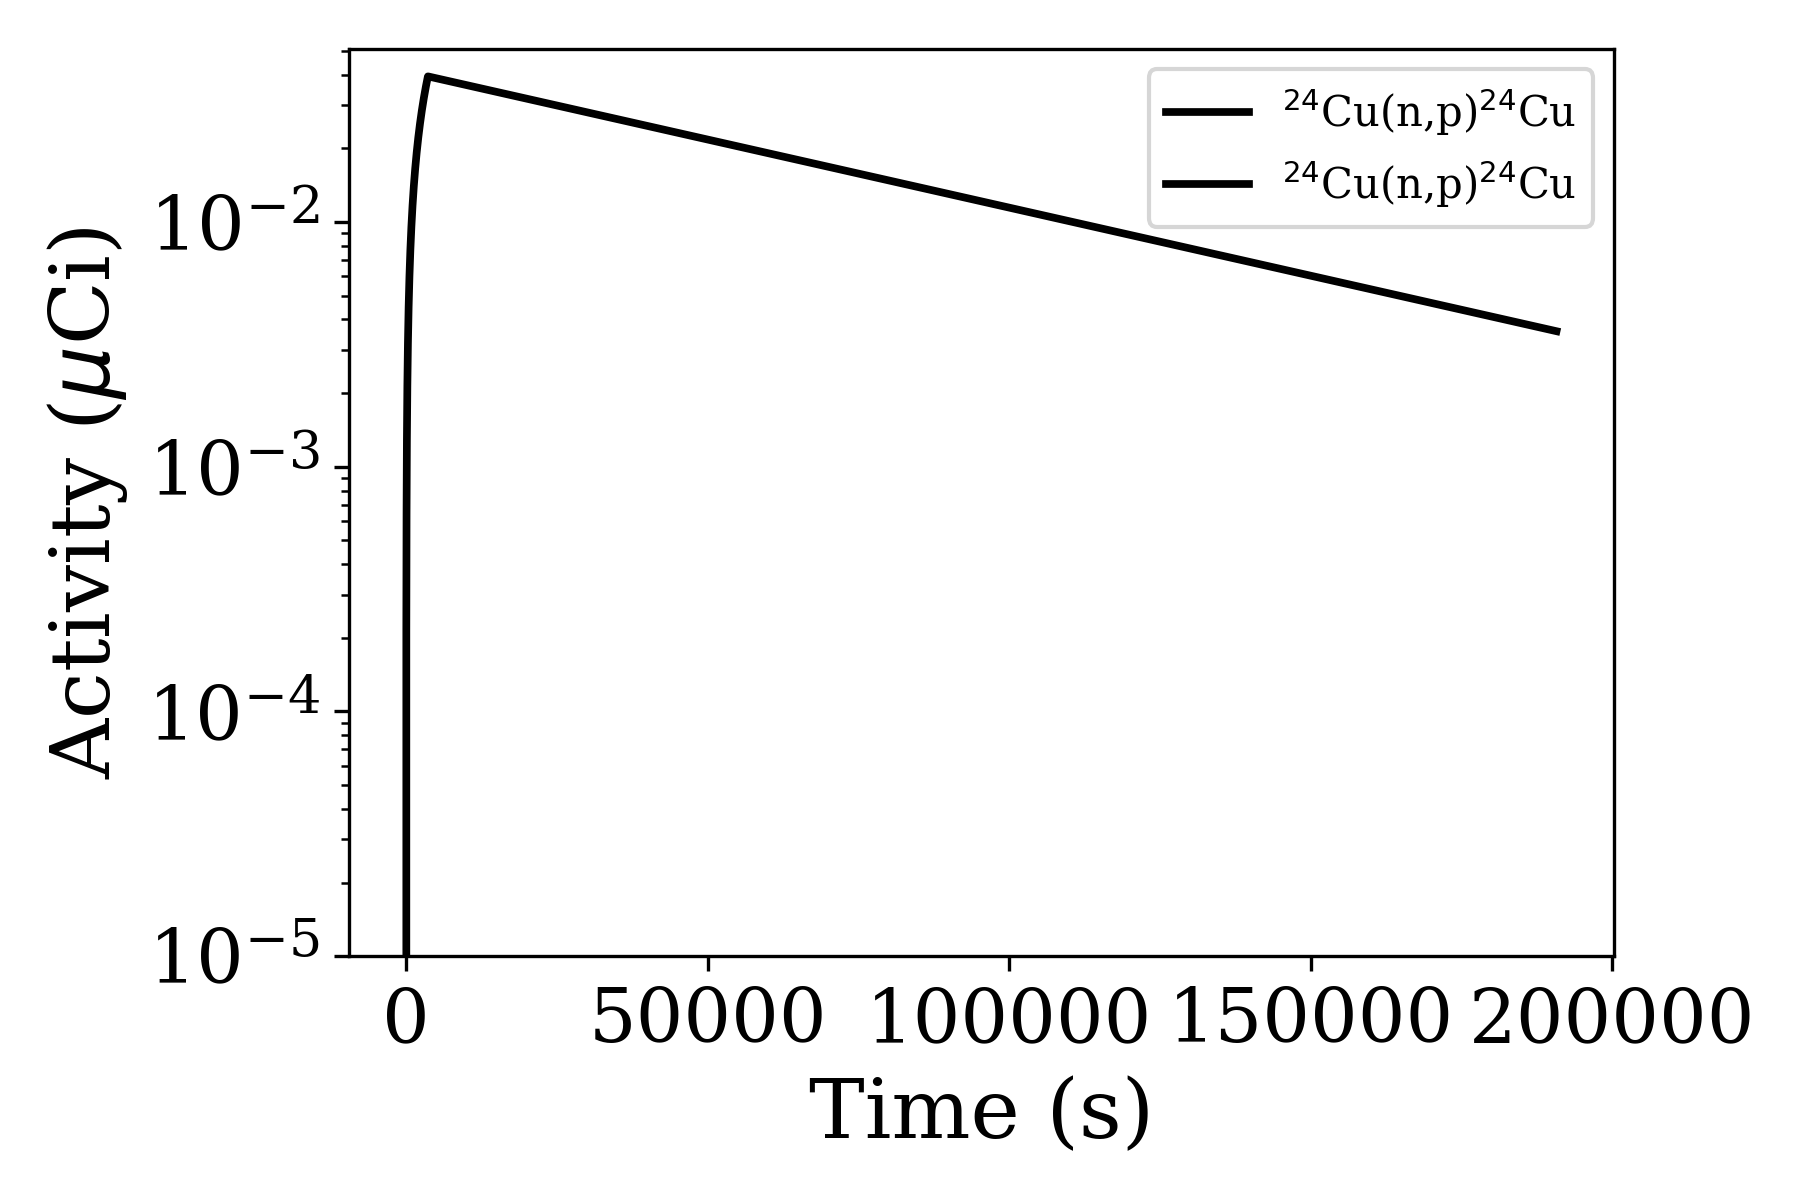
\includegraphics[width=.4\textwidth]{source/plot/Cu-24(n,p)Na-24_wisconsin1.png} 

\end{figure}

\begin{figure}[!ht]
   \centering
   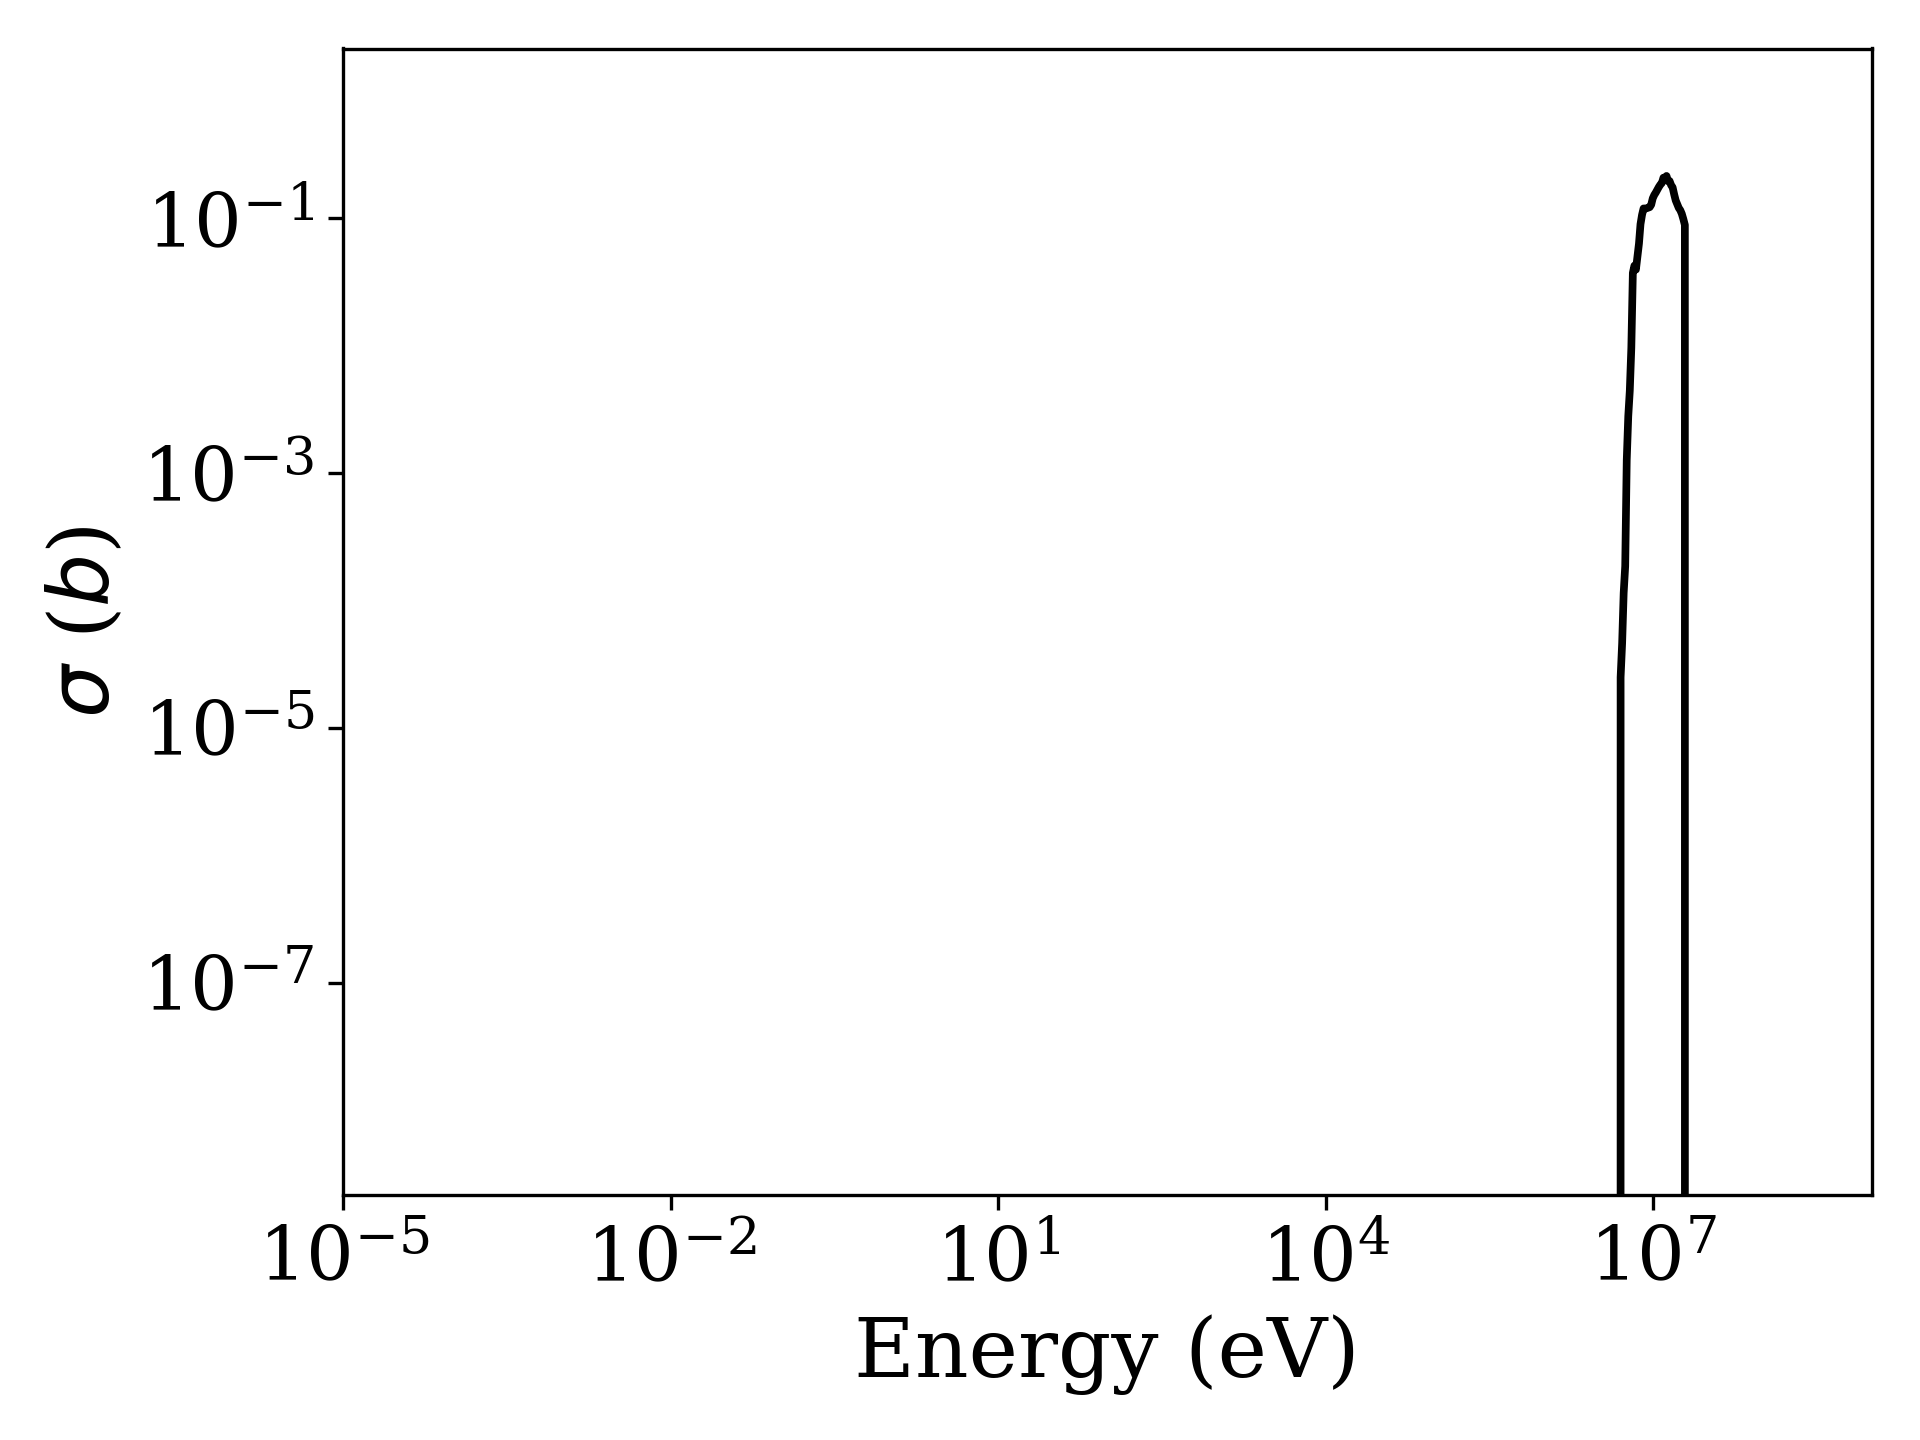
\includegraphics[width=.4\textwidth]{source/plot/Cu-24(n,p)Na-24.png} 

\end{figure}

\begin{table*}[h]
\centering
\begin{tabular}{ |c|c|c|c|c|c|c| }
 \hline
 Reaction & T$_{1/2}$ & ROI (eV) & Important Gammas (keV) \\
 \hline 
 $^{24}$Cu(n,p)$^{24}$Cu & 15.0 h & 6.46e+06, 1.18e+07 & 1368.626(0.999936),  \\ 
\hline
\end{tabular}
\end{table*}
